% 本章原书节号用阿拉伯数字；本章与 ch12b.tex 共用同一章，章末由 ch12b 恢复罗马数字，本章原书无参考文献表
\renewcommand{\thesection}{\arabic{section}}
\chapter{超越镜像对称}
\chapterauthor{中島啓}{[京都大学数理解析研究所]}

% ===== PDF p.157 (原书 p.149) =====
镜像对称的好处之一是，可以把有理曲线计数这一困难问题，替换成镜像的另一流形的变形这一（比较）容易的问题来求解。本章以“超越镜像对称”为题，想介绍关于计算 Gromov--Witten 不变量这一问题的近期显著进展。有理曲线计数问题相当于 Gromov--Witten 不变量中亏格为 0 的情形，而这里也处理亏格较高的情形。此外，纽结理论、表示论等数学上看来关系不大的各种领域，通过物理中弦论的对偶性而联系起来，出现了这样有趣的图景。也可以说，这是镜像对称的进一步深化，而镜像对称可看作辛几何与代数几何之间的对偶性。

Andrei Okounkov 在 ICM 2006 获得菲尔兹奖的事记忆犹新，获奖理由之一与 Gromov--Witten 不变量有关的一系列研究，其中一部分也与此相关。

\section{Gromov--Witten 不变量的母函数}

第 2 章（原书 p.18）有 Gromov--Witten 不变量的说明。简单复习一下。对 $\beta\in H_{2}(X,\Z)$，把亏格 $g$ 的黎曼面 $C$ 到 $X$ 的（稳定）全纯曲线所成的模空间记作 $\overline{M}_{g}(X,\beta)$。这时，Gromov--Witten 不变量是：把 $X$ 的上同调类拉回所得的上同调类，在 $\overline{M}_{g}(X,\beta)$ 上积分来定义的。更准确地说，不是通常的单纯积分，而是与称为虚拟基本类的 $[\overline{M}_{g}(X,\beta)]^{\mathrm{vir}}$ 这一同调类的元素取配对。

% ===== PDF p.158 (原书 p.150) =====
这是因为 $\overline{M}_{g}(X,\beta)$ 带有奇点、为了定义“正确”的积分而引入的；这里不作深入。

下面进一步把 $X$ 设为 3 维 Calabi--Yau 流形。应用 Hirzebruch--Riemann--Roch 定理，可以得到 $\overline{M}_{g}(X,\beta)$ 的（虚拟）维数不依赖于 $g$ 与 $\beta$、总是 0 这一性质。因此，Gromov--Witten 不变量 $N_{g,\beta}$ 定义为
\[ N_{g,\beta}=\int_{[\overline{M}_{g}(X,\beta)]^{\mathrm{vir}}}1. \]

$\overline{M}_{g}(X,\beta)$ 的（虚拟）维数为 0 是显著的性质：若维数不是 3，或流形不是 Calabi--Yau 流形，那么除非特意选取 $\beta$、并另在 $X$ 的上同调类上设法，否则微分形式的次数与维数就对不上，定义式只能得 0。在这个意义上，Gromov--Witten 不变量与 $X$ 是 3 维 Calabi--Yau 流形非常相配，因此关于 Gromov--Witten 不变量有许多深刻结果。本章讲的内容也关于 3 维 Calabi--Yau 流形的 Gromov--Witten 不变量，但如开头所述，要考察所有亏格 $g$。于是，把对所有的 $\beta,g$ 的 Gromov--Witten 不变量 $N_{g,\beta}$ 的母函数表示为
\[ F_{GW}(X;\hbar,\Lambda)=\sum_{\beta}\sum_{g}N_{g,\beta}\hbar^{2g-2}\Lambda^{\beta}. \tag{1} \]
$\Lambda,\hbar$ 分别是母函数中对应于全纯映射的次数与定义域黎曼面的亏格的变量。

通常，几何学家认为黎曼面的亏格越大就越复杂、越困难。而且亏格不同的情形分别处理，所以取关于亏格的母函数这种想法通常是没有的。然而本章所介绍的，尽是“一取关于亏格的母函数，别的结构就浮现出来”这样的主张。在这个意义上，把黎曼面的亏格全部变动起来看，在这一整体之上存在着某种几何结构——这就是母空间的含义。这与“弦论是把 Feynman 图加粗后看到的东西”这一物理洞察（图 1）很好地吻合。Feynman 图本来是在有某个根本理论、把它关于参数作微扰展开时出现的东西。不过目前还不清楚，作为微扰展开而看到的弦论，其根本理论究竟是什么。

% ===== PDF p.159 (原书 p.151) =====
因此，与其说已经看清了它，不如说我们的目标是找到那个“根本理论”——这样说也许更贴切。

\begin{figure}[t]
\centering
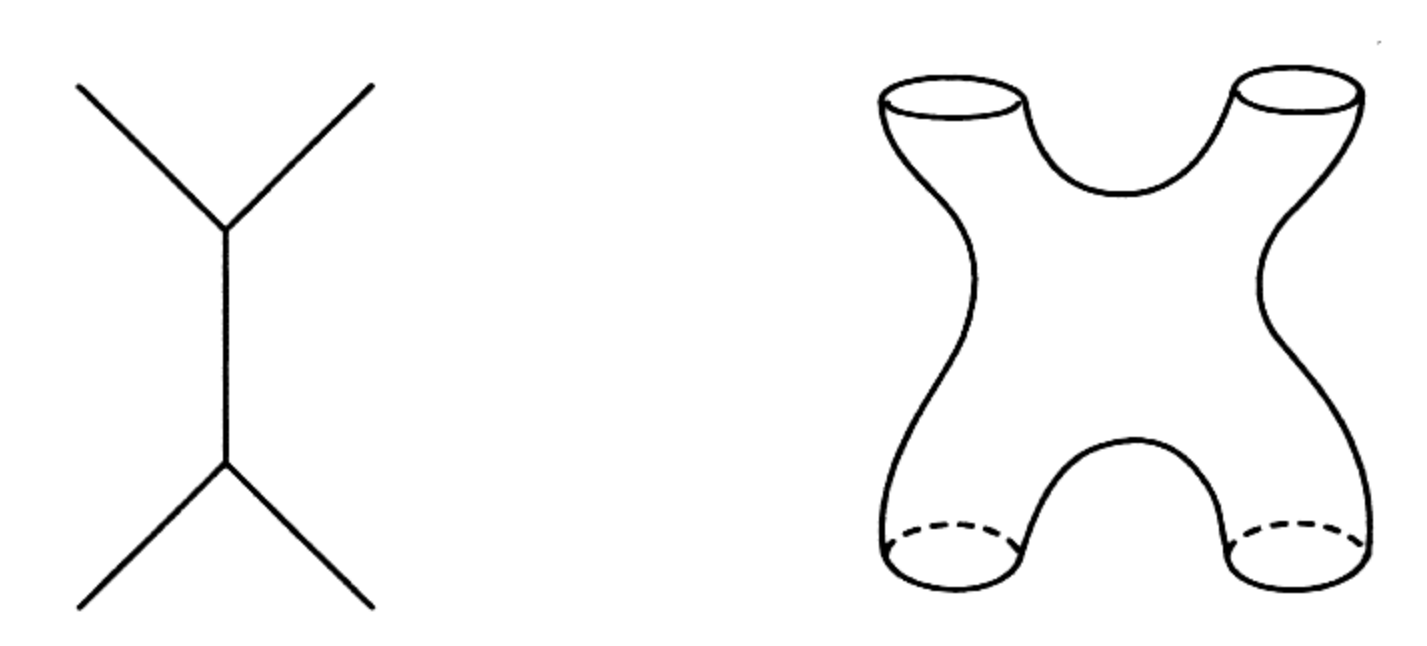
\includegraphics[width=0.58\linewidth]{figures/ch12-fig1.png}
\figtitle{1}{Feynman 图（左）与弦（右）（原书 p.151）}
\end{figure}

\section{局部镜像对称}

第 1 章（原书 p.15）简单介绍过“局部镜像对称”。这是研究非紧 Calabi--Yau 流形的 Gromov--Witten 不变量计算的工作。其中最基本的是称为锥形流形的奇点消解（resolved conifold）的东西，它考虑的是 $\PP^{1}$ 上第一 Chern 类为 $-1$ 的线丛 $\mathcal{O}(-1)$ 的两个直和 $\mathcal{O}(-1)\oplus\mathcal{O}(-1)$ 的全空间。

锥形流形的奇点消解之所以被大量研究，是因为紧 Calabi--Yau 流形中以“不动”的方式嵌入 $\PP^{1}$ 时，其近旁与这个空间相同。所谓不动，是说法丛没有全纯截面；选 $\mathcal{O}(-1)\oplus\mathcal{O}(-1)$ 这一 Chern 类，正是其反映。例如，Gromov--Witten 不变量的多重覆盖公式是表示这个空间的 Gromov--Witten 不变量的公式，由 Faber--Pandharipande 证明；人们认为，一般紧 Calabi--Yau 流形中以“不动”的方式嵌入 $\PP^{1}$ 时，其 $\PP^{1}$ 也会以同样的公式给出贡献，存在于 Gromov--Witten 不变量中。公式的具体形式是
\[ \sum_{g\ge 0}\frac{(-1)^{g-1}B_{2g}}{2g(2g-2)!}\sum_{d=1}^{\infty}d^{2g-3}\Lambda^{d}\hbar^{2g-2} \tag{2} \]
这样的东西。$\Lambda,\hbar$ 与 (1) 中相同，分别是母函数中对应于全纯映射的次数与定义域黎曼面的亏格的变量。$\hbar^{-2}$ 项对应来自 $S^{2}$ 的全纯映射，$\hbar^{0}$ 项对应来自环面的全纯映射。

% [Tutor Note: 原文「動かない」直译为“不动”，指该 $\PP^{1}$ 的法丛没有全纯截面、曲线不能变形，义近几何中的“刚性”（rigid）。]

% ===== PDF p.160 (原书 p.152) =====
不过，现在的情形可以看作到 $\PP^{1}$ 的映射，所以次数当作整数。其中 $B_{2g}$ 是 Bernoulli 数，由
\[ \frac{t}{e^{t}-1}=\sum_{n=0}^{\infty}\frac{B_{n}}{n!}t^{n} \]
给出。（$B_{0}=1$，$B_{1}=-1/2$，$B_{2}=1/6$，且 $g\ge 1$ 时 $B_{2g+1}=0$。）这个数例如也出现在 Hirzebruch 的 Riemann--Roch 公式中。它与本问题有没有关系尚不清楚，但从后面要说明的几何工程学看，它是自然的。

% [Tutor Note: 原文「幾何工学」是 geometric engineering 的日译，中文文献通行作“几何工程学”，此处照此译出。]

除此之外，$\PP^{1}\times\PP^{1}$ 的典范丛的全空间、$\PP^{2}$ 的典范丛的全空间等，紧流形上向量丛的全空间也是例子。后面的几何工程学中，还会出现以 $\PP^{1}$ 上的 ALE 空间（$\C^{2}/\Gamma$ 的奇点消解）为纤维的纤维丛等例子。

计算这些非紧 Calabi--Yau 流形的 Gromov--Witten 不变量时使用的有效工具，是关于环面作用的 Atiyah--Bott 不动点公式。一般而言，全纯曲线的模空间是并不清楚的空间，在其上执行上同调类的计算被认为很难；但由于模空间上有环面作用，积分便‘集中’到不动点上，计算就容易得多。这一手法也用于著名的 4 维射影空间 $\PP^{4}$ 中 5 次超曲面内有理曲线的计数。非紧 Calabi--Yau 流形的情形可进一步推进计算，最终凝结为拓扑顶点（topological vertex）理论。拓扑顶点是非常有趣的话题，但这里因篇幅关系只能割爱省略。

\section{大 N 相对性}

Gromov--Witten 不变量以及更早定义的 Donaldson 不变量，与模空间的几何相关联而得到活跃研究。另一方面，与它们性质稍有不同的、同样被活跃研究的不变量，有基于 Chern--Simons 理论的称为纽结不变量的东西。这个不变量有各种版本，最初的一个是原本与纽结理论毫无关系的算子代数专家
% ===== PDF p.161 (原书 p.153) =====
Jones 发现的不变量，称为 Jones 不变量。后来，针对 Atiyah 提出的“用场论解释 Jones 不变量”这一问题，理论物理学家 Witten 回答说，可以把 Chern--Simons 泛函在联络全体所成的无穷维空间上作路径积分来定义。于是，它作为关于 3 维流形中纽结的 Jones--Witten 不变量，在更大的框架中被定式化。关于这个理论有许多有趣的话题，有兴趣的读者请看《量子不变量——三维拓扑与数理物理的相遇》（大槻知忠 编，日本評論社，2002）。这里要强调的是，它与 Gromov--Witten 不变量性质不同。理由是：Gromov--Witten 不变量是作为模空间上的积分来定义的不变量，而 Jones--Witten 不变量是作为联络全体所成的无穷维空间上的路径积分来定义的不变量。前者是并不清楚的模空间上的积分，但毕竟是有限维流形上的积分，可以数学上严格定义；后者则基于路径积分这一数学上没有基础的东西。

实际上，Jones--Witten 不变量在数学上的严格定义由 Reshetikhin--Turaev 与河野俊丈给出，但不是实际执行积分，而是用间接手法给出的。Witten 在“路径积分可以定义、并具有与有限维积分相似性质”这一假设之下，导出了计算不变量的算法。他把这个算法当作定义来采用，并证明无论用哪种计算方式答案总相同，从而给出了定义。
% [Tutor Note: 原书此处作「ラージ N 相対性」。按内容（Gopakumar--Vafa 1998 年的结果）通常称为 large N duality，即大 N 对偶；此处照原题译作“大 N 相对性”。]

大 N 相对性主张这两个性质不同的纽结不变量与 Gromov--Witten 不变量之间存在联系，由物理学家 Gopakumar--Vafa 于 1998 年发现。这里 $N$ 表示定义 Chern--Simons 泛函所考虑的联络的主丛的结构群为 $U(N)$，并对所有的 $N$ 同时考虑。其想法基于 't Hooft 1974 年的主张：$U(N)$ 规范理论的 $N\to\infty$ 极限与弦论等价。

取最简单的 $S^{3}$ 作为 3 维流形。先考虑纽结为空集的情形下的 Jones--Witten 不变量（这样的东西也是允许的）。

% ===== PDF p.162 (原书 p.154) =====
结构群采用 $U(N)$，给出正整数 $k$（称为水平）。这时，Jones--Witten 不变量等于对 (1) 的母函数取指数所得，这就是 Gopakumar--Vafa 的结果。不过，把 $N$ 与 $k$ 看作变量，把 Gromov--Witten 不变量的母函数 (1) 中出现的变量读作
\[ \hbar=\frac{2\pi}{k+N},\qquad \Lambda=\exp\left(-\frac{2\pi\sqrt{-1}N}{k+N}\right) \]
主张不变量相等。这个主张本身，因为两边的不变量都有数学上严格的定义，只要计算两边并观察其相等便可确认。但是，为什么这样的事会成立，其物理解说中含有令人惊叹的想法，而这在数学上尚未被严格正当化。

下面说明其想法。首先，为什么实 3 维流形的 $S^{3}$ 与复 3 维流形的锥形流形奇点消解之间有关系，这基于 Witten 1992 年的主张“Chern--Simons 理论是弦论”。$S^{3}$ 的余切丛 $X=T^{*}S^{3}$ 具有复结构，把它看作非紧 Calabi--Yau 流形。这时，

1. $S^{3}$ 的 Jones--Witten 不变量

2. 由带边黎曼面到 $T^{*}S^{3}$ 的全纯映射所构成的 Gromov--Witten 不变量

相等，这就是 Witten 的主张。通常的 Gromov--Witten 不变量，是作为从无边界黎曼面出发的全纯映射的模空间 $\overline{M}_{g}(X,\beta)$ 上的积分来定义的。把它推广：定义域的黎曼面允许带边界，把边界送入 $S^{3}$ 的全纯映射全体汇集起来作模空间，用同样的积分来定义不变量。不过，据说基于来自亏格更高的带边黎曼面的全纯映射来定义 Gromov--Witten 不变量，技术上有微妙的问题\footnote{承蒙深谷賢治、小野薫告知。}，数学上还没有给出严格定义。而且，现在的情形若单纯考虑全纯映射，则只有常值映射，如何定义不变量需要慎重考察。

% ===== PDF p.163 (原书 p.155) =====
其次，把 $T^{*}S^{3}$ 与锥形流形的奇点消解联系起来。这是 3 维 Calabi--Yau 流形中常见的手法，即第 4 章中並河说明的锥形流形跃迁。虽是重复说明，但现在的情形可以具体做出来。首先，锥形流形是 $\C^{4}$ 中由 $\{xy=uv\}$ 定义的、在原点有奇点的超平面。把它按 $xy=uv-\mu$ 用参数 $\mu$ 变形，容易看出它与 $T^{*}S^{3}$ 微分同胚。另一方面，作为奇点消解可以取第 2 节开头所述的 $\mathcal{O}(-1)\oplus\mathcal{O}(-1)$。实际上，从它到锥形流形的映射由
\[ \mathcal{O}(-1)\oplus\mathcal{O}(-1)\ni([z_{0}:z_{1}],\xi,\zeta)\mapsto(x,y,u,v)=(\xi z_{0},\zeta z_{1},\zeta z_{0},\xi z_{1}) \]
给出。其中 $[z_{0}:z_{1}]$ 是底空间的射影直线的坐标，$\xi,\zeta$ 是线丛 $\mathcal{O}(-1)$ 的纤维坐标。

Gopakumar--Vafa 洞察到：通过锥形流形跃迁，前面的 2 的不变量与

3. 从无边界黎曼面到锥形流形奇点消解的 Gromov--Witten 不变量

相等。要注意：如第 2 节所述，第 3 项（作为不变量）在数学上有严格定义，这一点与第 2 项的不变量在数学定义上仍留有模糊之处大不相同。因此，“第 1 项的不变量与第 3 项的不变量相等”这一主张在数学上有意义。而且，只要把两边都算出来，该主张确实成立。

Gopakumar--Vafa 的这一发现被大栗--Vafa 深化。此前的考察是没有纽结时 $S^{3}$ 的 Jones--Witten 不变量，而有纽结（链环）$L$ 时可作如下扩张。首先，1 的不变量本来就在有 $L$ 的情形下有定义。2 的不变量替换为

2'. 从带边黎曼面到 $T^{*}S^{3}$ 的全纯映射中，边界落在 $S^{3}$ 与 $L$ 的余法丛中的全纯映射所构成的 Gromov--Witten 不变量。

% [接续: PDF p.163 末项 2'. 的句子「2 の不变量は 2'. ……不変量」收尾在 p.164 顶部「で置き換えられます」，本文件已补成「……的 Gromov--Witten 不变量。」；p.164 第一段从「そして，コニフォールド・トランジションを通じて $L$ の余法束が，コニフォールドの特異点解消の中のラグランジアン部分多様体 $\mathcal{L}_{L}$ を定めると予測します．」起，由 ch12b.tex 续写]
